

\chapter{Code}


All written code for this project can be found on Github at \url{https://github.com/TimToernes/MGA-PyPSA}. 


\subsection{Pseudo code}

\begin{enumerate}[label={}]
\item Solve network subject to regular constraints and with original objective function
\item Add MGA constraint !Equation number
\item while $\epsilon>tol$
\begin{itemize}[label={}]
\item If first loop
\begin{itemize}[label={}]
\item directions = max and min all variables
\end{itemize}
\item Else
\begin{itemize}[label={}]
\item directions = normals to hull faces
\end{itemize}
\item for direction in directions
\begin{itemize}[label={}]
\item objective function = direction[i] * variable[i]
\item point on convex hull += solve problem subject to objective function
\end{itemize}
\item hull = ConvexHull ( points on convex hull)
\item $epsilon$ = new hull volume - old hull volume / hull volume
\end{itemize}
\item Evenly distribute points in hull 
\item Plot histogram using evenly distributed points. 
\end{enumerate}




\chapter{Plots for section \ref{sec:4D} }

\begin{figure}[p]\center
	\includegraphics[width=1.2\textwidth,trim={0 0cm 0 0cm},clip]{./Images/corelation_4D_00}
	\caption{Variable correlations of the MGA study with a CO2 emission reduction of 0\%. Distributions of the four individual technologies are plotted on the diagonal.}

\end{figure}

\begin{figure}[p]\center
	\includegraphics[width=1.2\textwidth,trim={0 0cm 0 0cm},clip]{./Images/corelation_4D_50}
	\caption{Variable correlations of the MGA study with a CO2 emission reduction of 50\%. Distributions of the four individual technologies are plotted on the diagonal.}

\end{figure}

\begin{figure}[p]\center
	\includegraphics[width=1.2\textwidth,trim={0 0cm 0 0cm},clip]{./Images/corelation_4D_80}
	\caption{Variable correlations of the MGA study with a CO2 emission reduction of 80\%. Distributions of the four individual technologies are plotted on the diagonal.}

\end{figure}

\begin{figure}[p]\center
	\includegraphics[width=1.2\textwidth,trim={0 0cm 0 0cm},clip]{./Images/corelation_4D}
	\caption{Variable correlations of the MGA study with a CO2 emission reduction of 95\%. Distributions of the four individual technologies are plotted on the diagonal.}

\end{figure}




\begin{figure}[p]\raggedleft
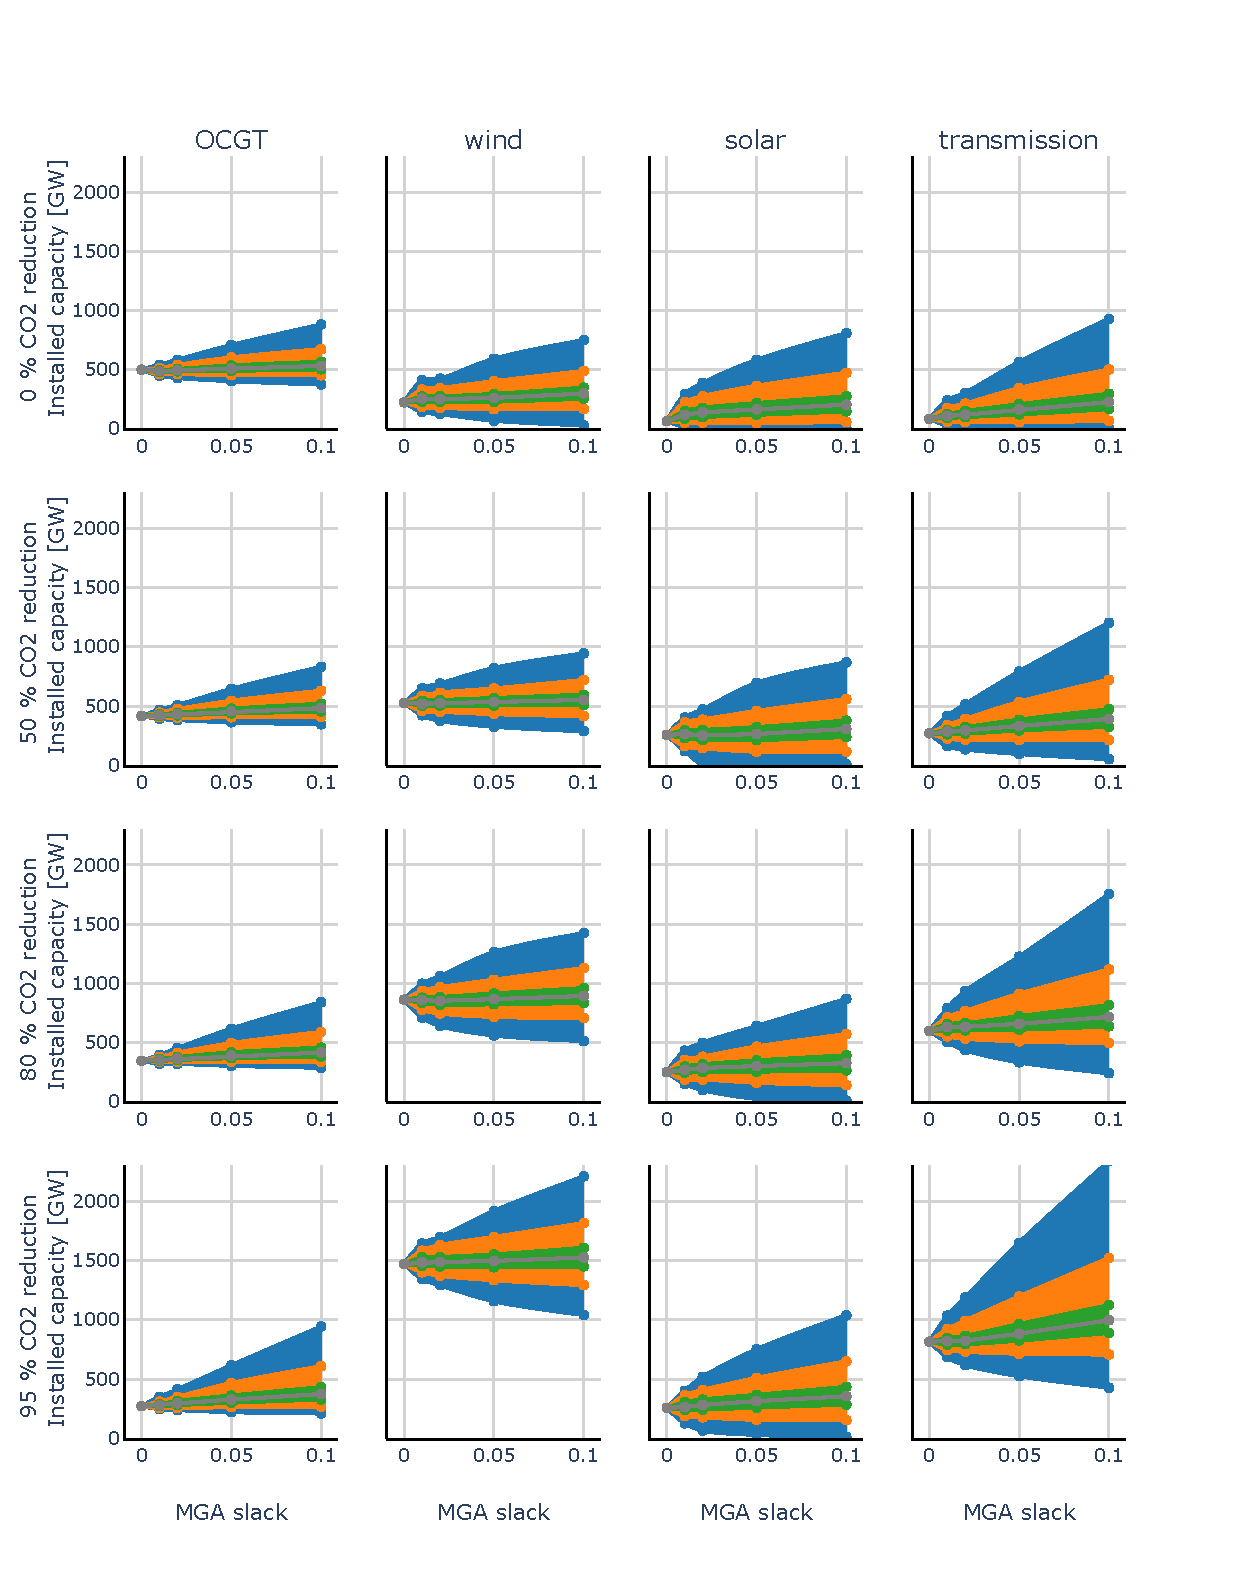
\includegraphics[width=.9\paperwidth,trim={0 0cm 0 0cm},clip]{./Images/Capacaty_vs_cost}
\label{fig:cap_vs_cost}
\caption{text}
\end{figure}
